\documentclass[tikz,border=5mm]{standalone}
\usepackage[utf8]{vietnam}
\usepackage{pgfplots}
\usetikzlibrary{calc,patterns,fillbetween}
%==============

\begin{document}
	%%%%%%%%%%%%%%%%%%%%%%%
	
	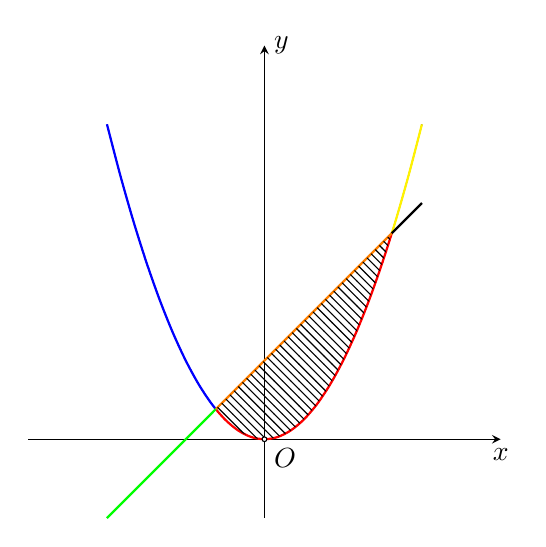
\begin{tikzpicture}
		\draw[-stealth] (-3,0)--(3,0) node[below]{$x$};
		\draw[-stealth] (0,-1)--(0,5) node[right]{$y$};
		\draw[smooth,name path=hsf] plot[domain=-2:2] (\x,{(\x)^2});
		\draw[name path=hsg] plot[domain=-2:2] (\x,{\x+1});
		\draw[blue,thick, intersection segments={of=hsf and hsg,sequence=L1}];
		\draw[red,thick, intersection segments={of=hsf and hsg,sequence=L2}];
		\draw[yellow,thick, intersection segments={of=hsf and hsg,sequence=L3}];
		\draw[black,thick, intersection segments={of=hsg and hsf,sequence=L3}];
		\draw[orange,thick, intersection segments={of=hsg and hsf,sequence=L2}];
		\draw[green,thick, intersection segments={of=hsg and hsf,sequence=L1}];
		\fill[pattern=north west lines,intersection segments={of=hsf and hsg,sequence=L2}][intersection segments={of=hsf and hsg,sequence=R2}];
		\draw[fill=white] (0:0) circle (.03) node[below right]{$O$};
	\end{tikzpicture}
	
	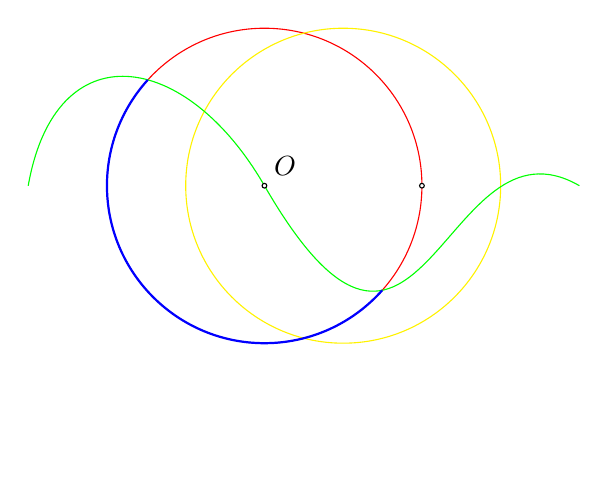
\begin{tikzpicture}
		\draw[red,name path=c1] (0:0) circle (2);
		\draw[yellow,name path=c2] (0:1) circle (2);
		\draw[green,name path=con] 
		(180:3) .. controls +(80:2) and +(120:2) .. (0,0)
		.. controls +(-60:4) and +(150:2) .. (0:4)
		;
		\draw[blue,thick, intersection segments={of=con and c1,sequence=R2}];
		\draw[fill=white] 
		(0:0) circle (.03) node[above right]{$O$}
		(0:2) circle (.03)
		;
	\end{tikzpicture}
	%=============
\end{document}